
\documentclass{beamer}
\usepackage[10pt]{extsizes} 
\usepackage[T2A]{fontenc}
\usepackage[utf8]{inputenc}
\usepackage[english,russian]{babel}
%\usepackage{pscyr}
\usepackage{hyperref}
\usepackage{setspace}
\usepackage{amsmath,amssymb,amsfonts,amsthm,secdot}

\usetheme{focus} % Use the Focus theme supplied with the template
% Add option [numbering=none] to disable the footer progress bar
% Add option [numbering=fullbar] to show the footer progress bar as always full with a slide count

% Uncomment to enable the ice-blue theme
%\definecolor{main}{RGB}{92, 138, 168}
%\definecolor{background}{RGB}{240, 247, 255}

\usepackage{booktabs} % Required for better table rules

%----------------------------------------------------------------------------------------
%	 TITLE SLIDE
%----------------------------------------------------------------------------------------

\title{Тема: \\ Трассировка лучей }

\subtitle{}

\author{Михайлин Д.А.}



\date{02.05.2019}

%------------------------------------------------

\begin{document}

%------------------------------------------------

\begin{frame}
	\maketitle 
\end{frame}

%----------------------------------------------------------------------------------------
%	 SECTION 1
%----------------------------------------------------------------------------------------

\section{Основные понятия.} % Section title slide, unnumbered

%------------------------------------------------

\begin{frame}{Поток}
	\begin{columns}
		\column{0.5\textwidth}
			Поток излучения обозначается - $\Phi$(Flux). 
		
		\column{0.5\textwidth}
			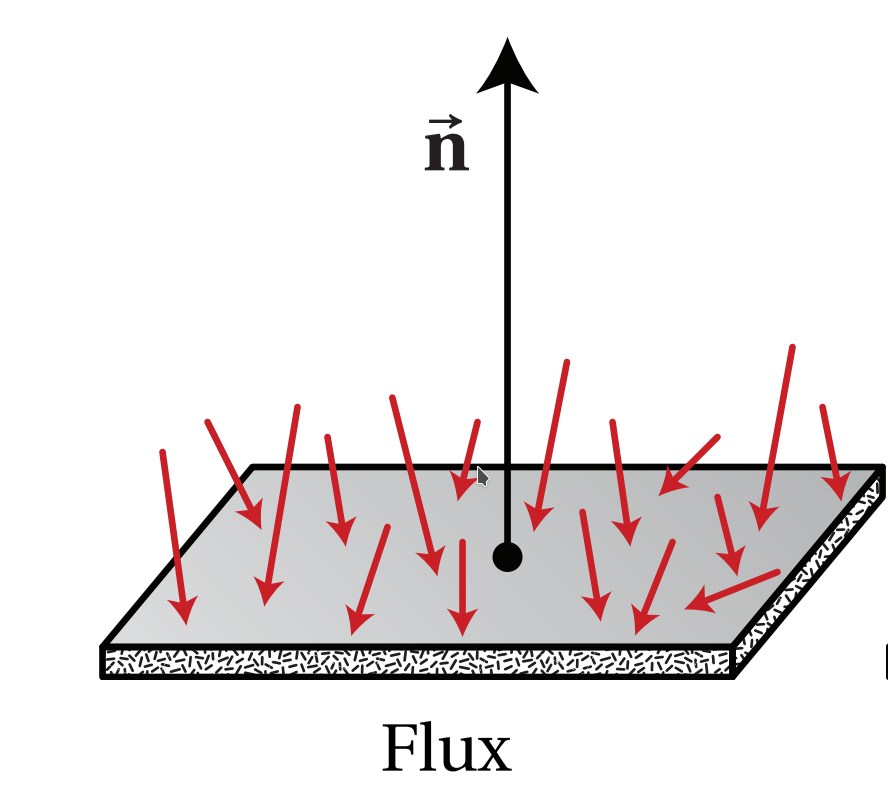
\includegraphics[width=\linewidth]{Flux.png}
	\end{columns}
\end{frame}

\begin{frame}{Интенсивность излучения}
	\begin{columns}
		\column{0.5\textwidth}
			Интенсивность излучения обозначается - E(Irradiance). $E = \frac{d\Phi(x)}{dS(x)}$
		
		\column{0.5\textwidth}
			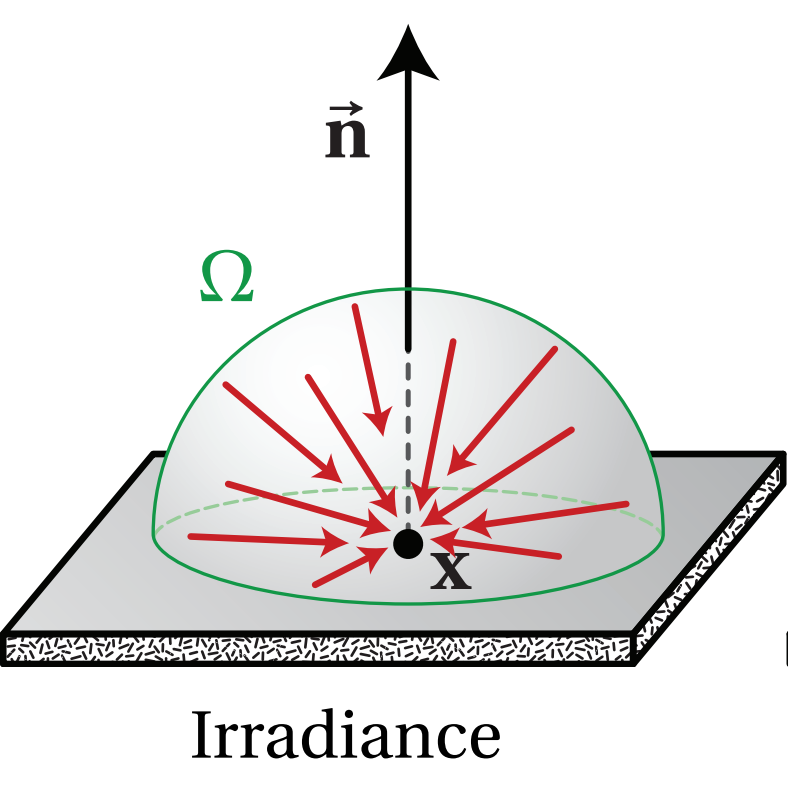
\includegraphics[width=\linewidth]{Irradiance.png}
	\end{columns}
\end{frame}
\begin{frame}{Cветимость}
	\begin{columns}
		\column{0.5\textwidth}
			Светимость обозначается - L(Radiance).\\ $L(x, \omega) = \frac{d^2\Phi(x)}{d\omega(x)dA^{\perp}(x)}$ \\ Можно переписать это уравнение в виде: \\$L(x, \omega) = \frac{d^2\Phi(x)}{d\omega(x)dA(x)(\omega, n)} = \frac{d^2\Phi(x)}{d\omega^{\perp}(x)dA(x)}$ 
		
		\column{0.5\textwidth}
			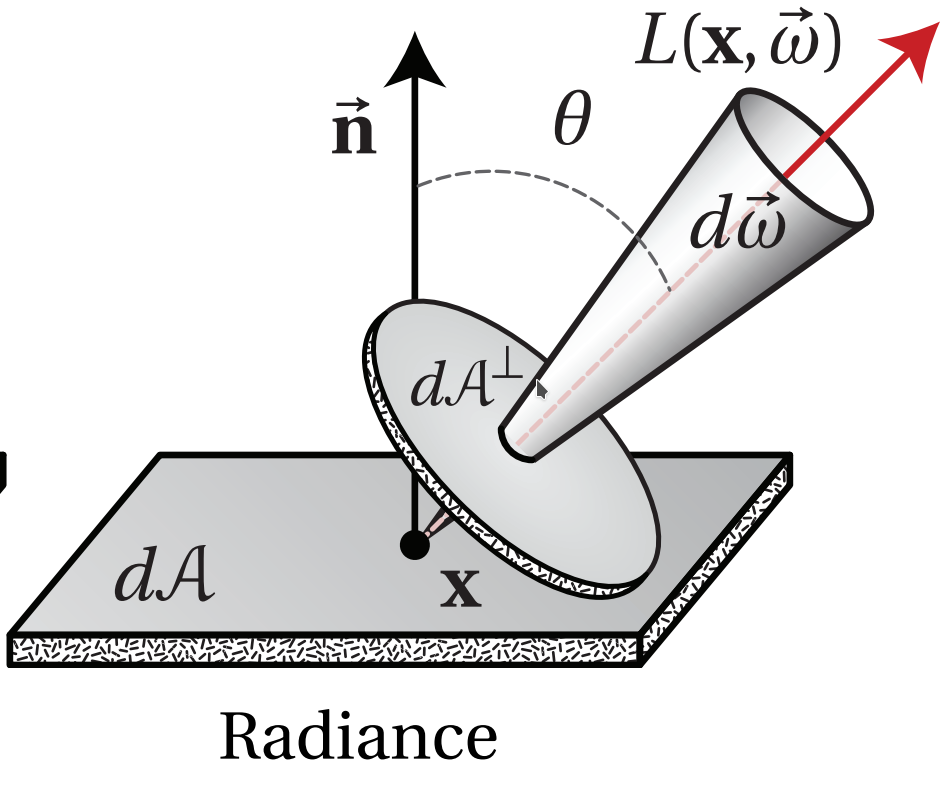
\includegraphics[width=\linewidth]{Radiance.png}
	\end{columns}
\end{frame}

\begin{frame}{Cвязь между этими величинами:}
	$L(x, \omega) = \frac{d^2\Phi(x)}{d\omega(x)dA^{\perp}(x)}$;\\ $L(x, \omega)d\omega(x)dA^{\perp}(x) = d^2\Phi(x)$;\\ $\Phi(x) = \int_A \int_{\Omega} L(x, \omega)d\omega(x)dA^{\perp}(x)$ = $\int_A \int_{\Omega} L(x, \omega)(\omega, n)d\omega(x)dA(x)$ \\ Получили выражение для потока через светимость. \\ 
	Также можем выразить интенсивность излучения через светимость. \\
	$E(x) = \int_{\Omega}L(x,\omega)(\omega, n)d\omega = \int_{\Omega}L(x, \omega)d\omega^{\perp}$
	
\end{frame}

\begin{frame}{BRDF}
	Введем обозначения:\\
	$L(x\rightarrow\omega)$ - функция которая описывает поток, исходящий из точки х в направлении $\omega$.\\
	Bidirectional reflectance distribution function. Эта функция описывает насколько "ярко" выглядит поверхность с направления $\omega$.\\
	$f_r(x, \omega_1\rightarrow\omega) = \frac{dL(x\rightarrow\omega)}{dE(x\leftarrow\omega_1)} = \frac{dL(x\rightarrow\omega)}{L(x\leftarrow\omega_1)(n,\omega_1)d\omega_1}$
	
\end{frame}

\begin{frame}{Основное уравнение рендеринга.}
	Основное уравнение рендеринга выглядит следующим образом:\\
	$L(x\rightarrow\omega) = L_e(x\rightarrow\omega) + L_r(x\rightarrow\omega)$\\
	total outgoing = emmitted + reflected\\
	$L(x\rightarrow\omega) = L_e(x\rightarrow\omega) + \int_{\Omega}f_r(x,w \rightarrow w')L(x\leftarrow\omega')(n,\omega')d\omega'$
\end{frame}
\begin{frame}{Методы Монте-Карло}
	Рассмотрим интеграл вида $I = \int_a^b\phi(x)dx$. Введем случайную величину X, которая равномерно распределена. \\
	$E[\phi(x)] = \int_a^b\phi(x)f(x)dx = \frac{1}{b - a}\int_a^b\phi(x)dx$. Отсюда:
	\\$\int_a^b\phi(x)dx = (b - a)E[\phi(x)]$. Заменим математическое ожидание его оценкой - выборочным средней.
	\\$I^* = (b - a)\frac{\sum\limits_{i = 1}^N \phi(x_i)}{N}$
\end{frame}
\begin{frame}
	Для вычисления интеграла введем функцию f(x) - плотность распределения случайной величины X. \\
	$\int_a^bf(x)dx = 1$\\
	Представим интеграл в виде:\\
	$\int_a^b \frac{\phi(x)f(x)}{f(x)}dx$\\
	Т.е. интеграл представлен в виде математического ожидания функции $\frac{\phi(x)}{f(x)}$;
	Для оценки интеграла будем использовать выборочное среднее. \\
	$I^*_2 = \frac{1}{N}\sum\limits_{i = 1}^N\frac{\phi(x_i)}{f(x_i)}$ 
\end{frame}
\begin{frame}
	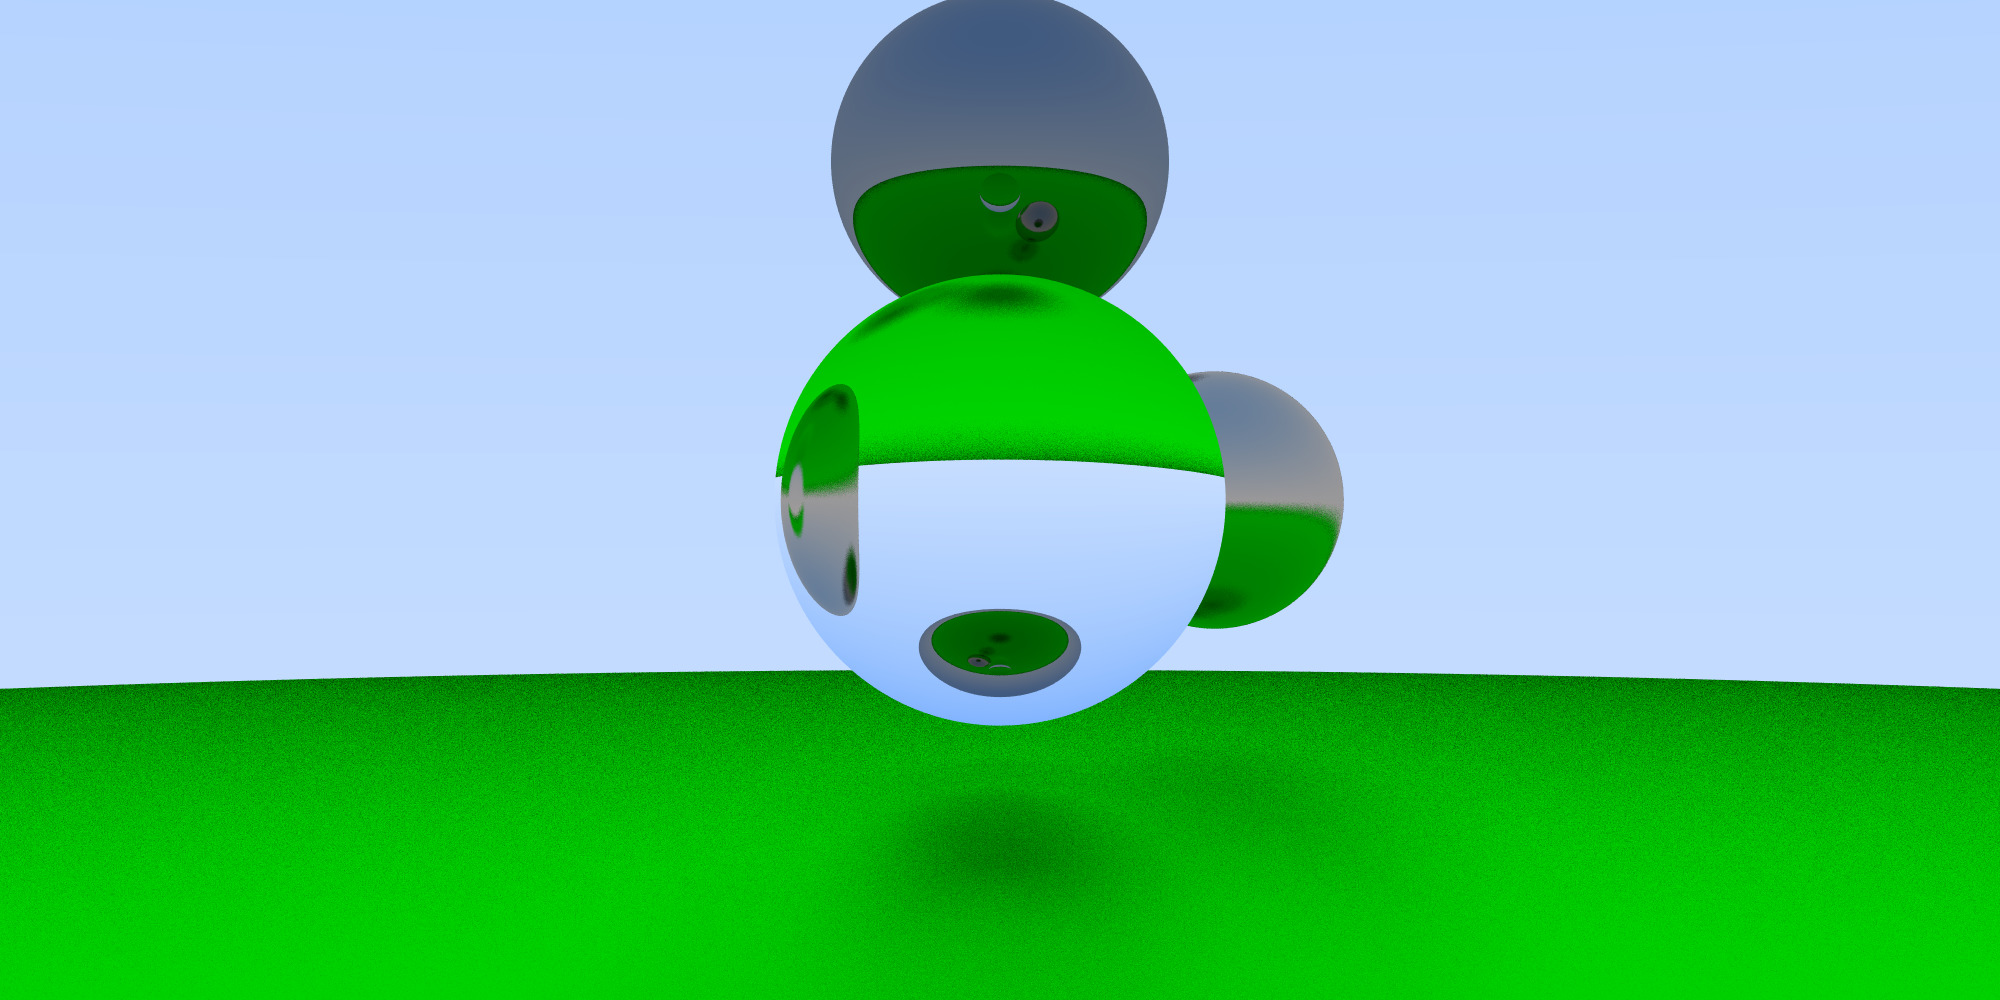
\includegraphics[width=\linewidth]{/home/dmitry/TestRT/wtf.jpg}
\end{frame}
\begin{frame}
	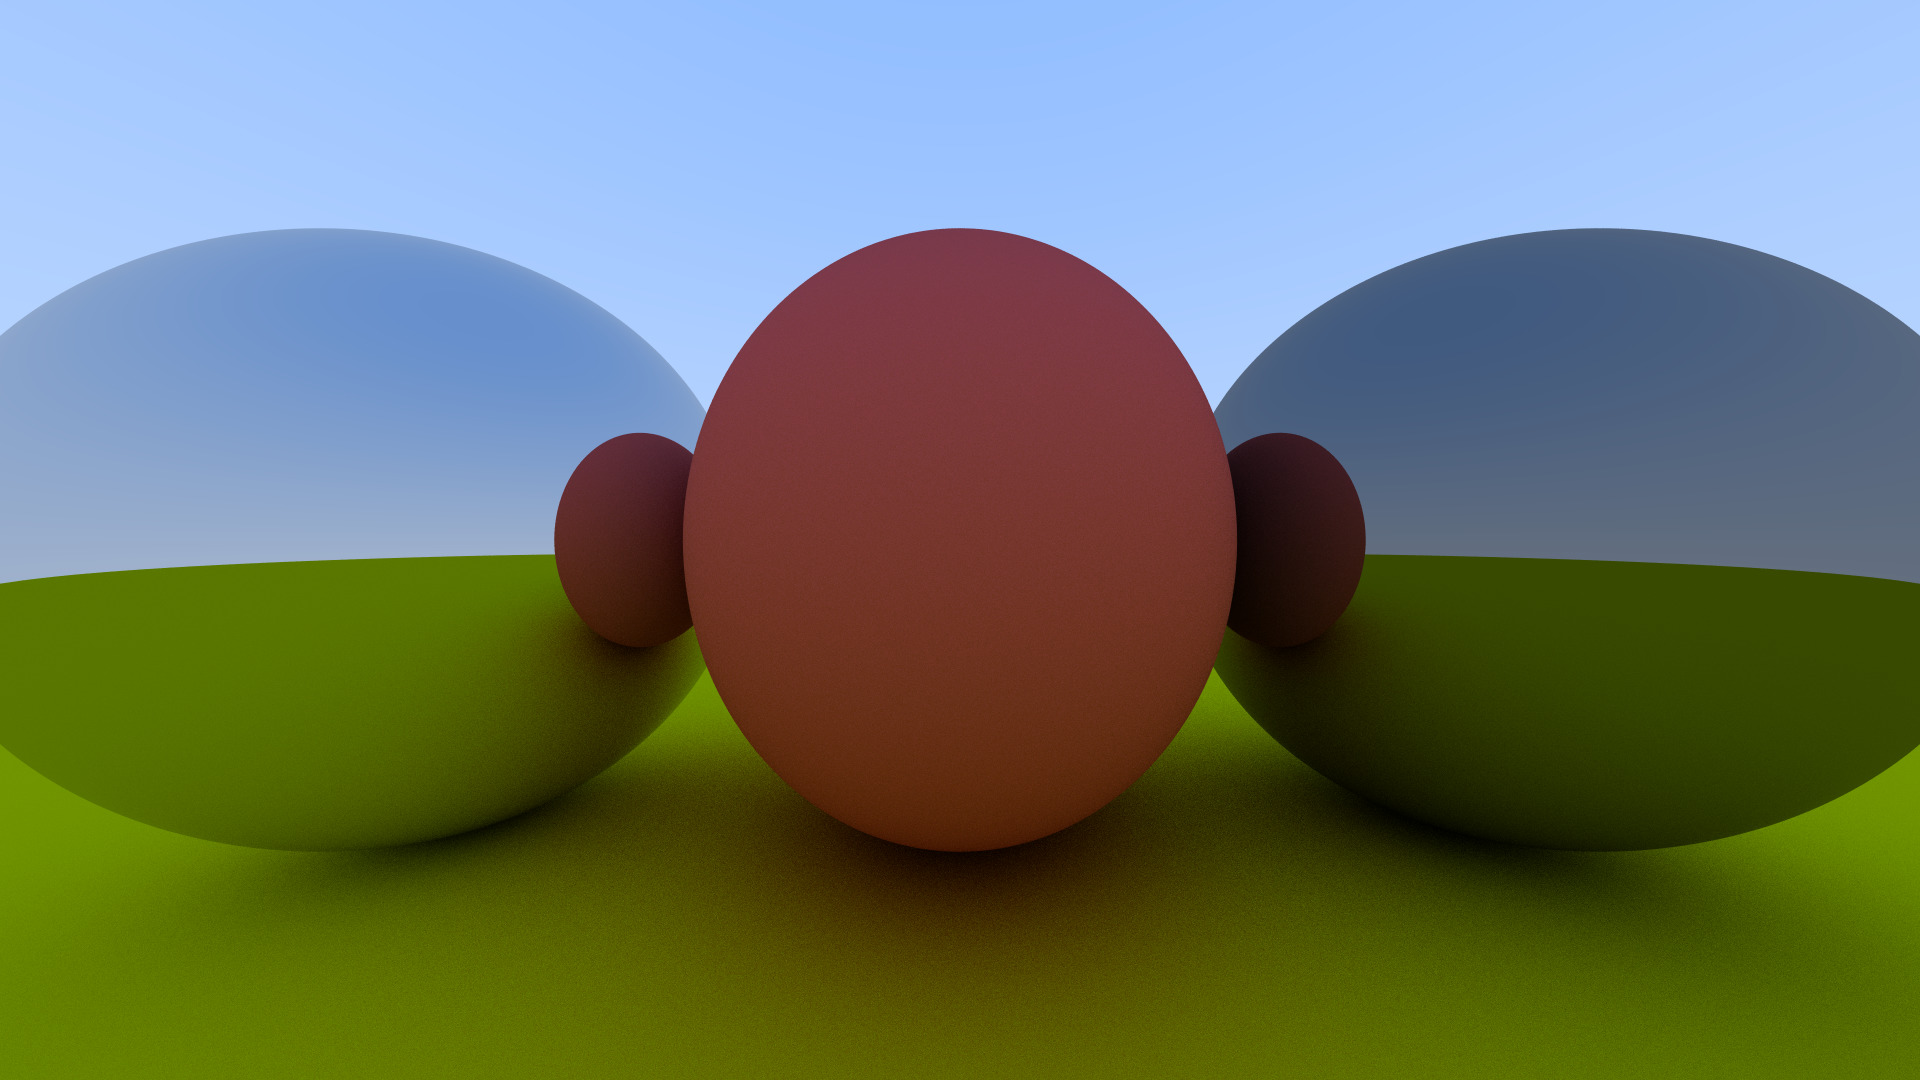
\includegraphics[width=\linewidth]{picture.jpg}
\end{frame}

\begin{frame}
	
\includegraphics[width=\linewidth]{metal.jpg}
\end{frame}

\begin{frame}
	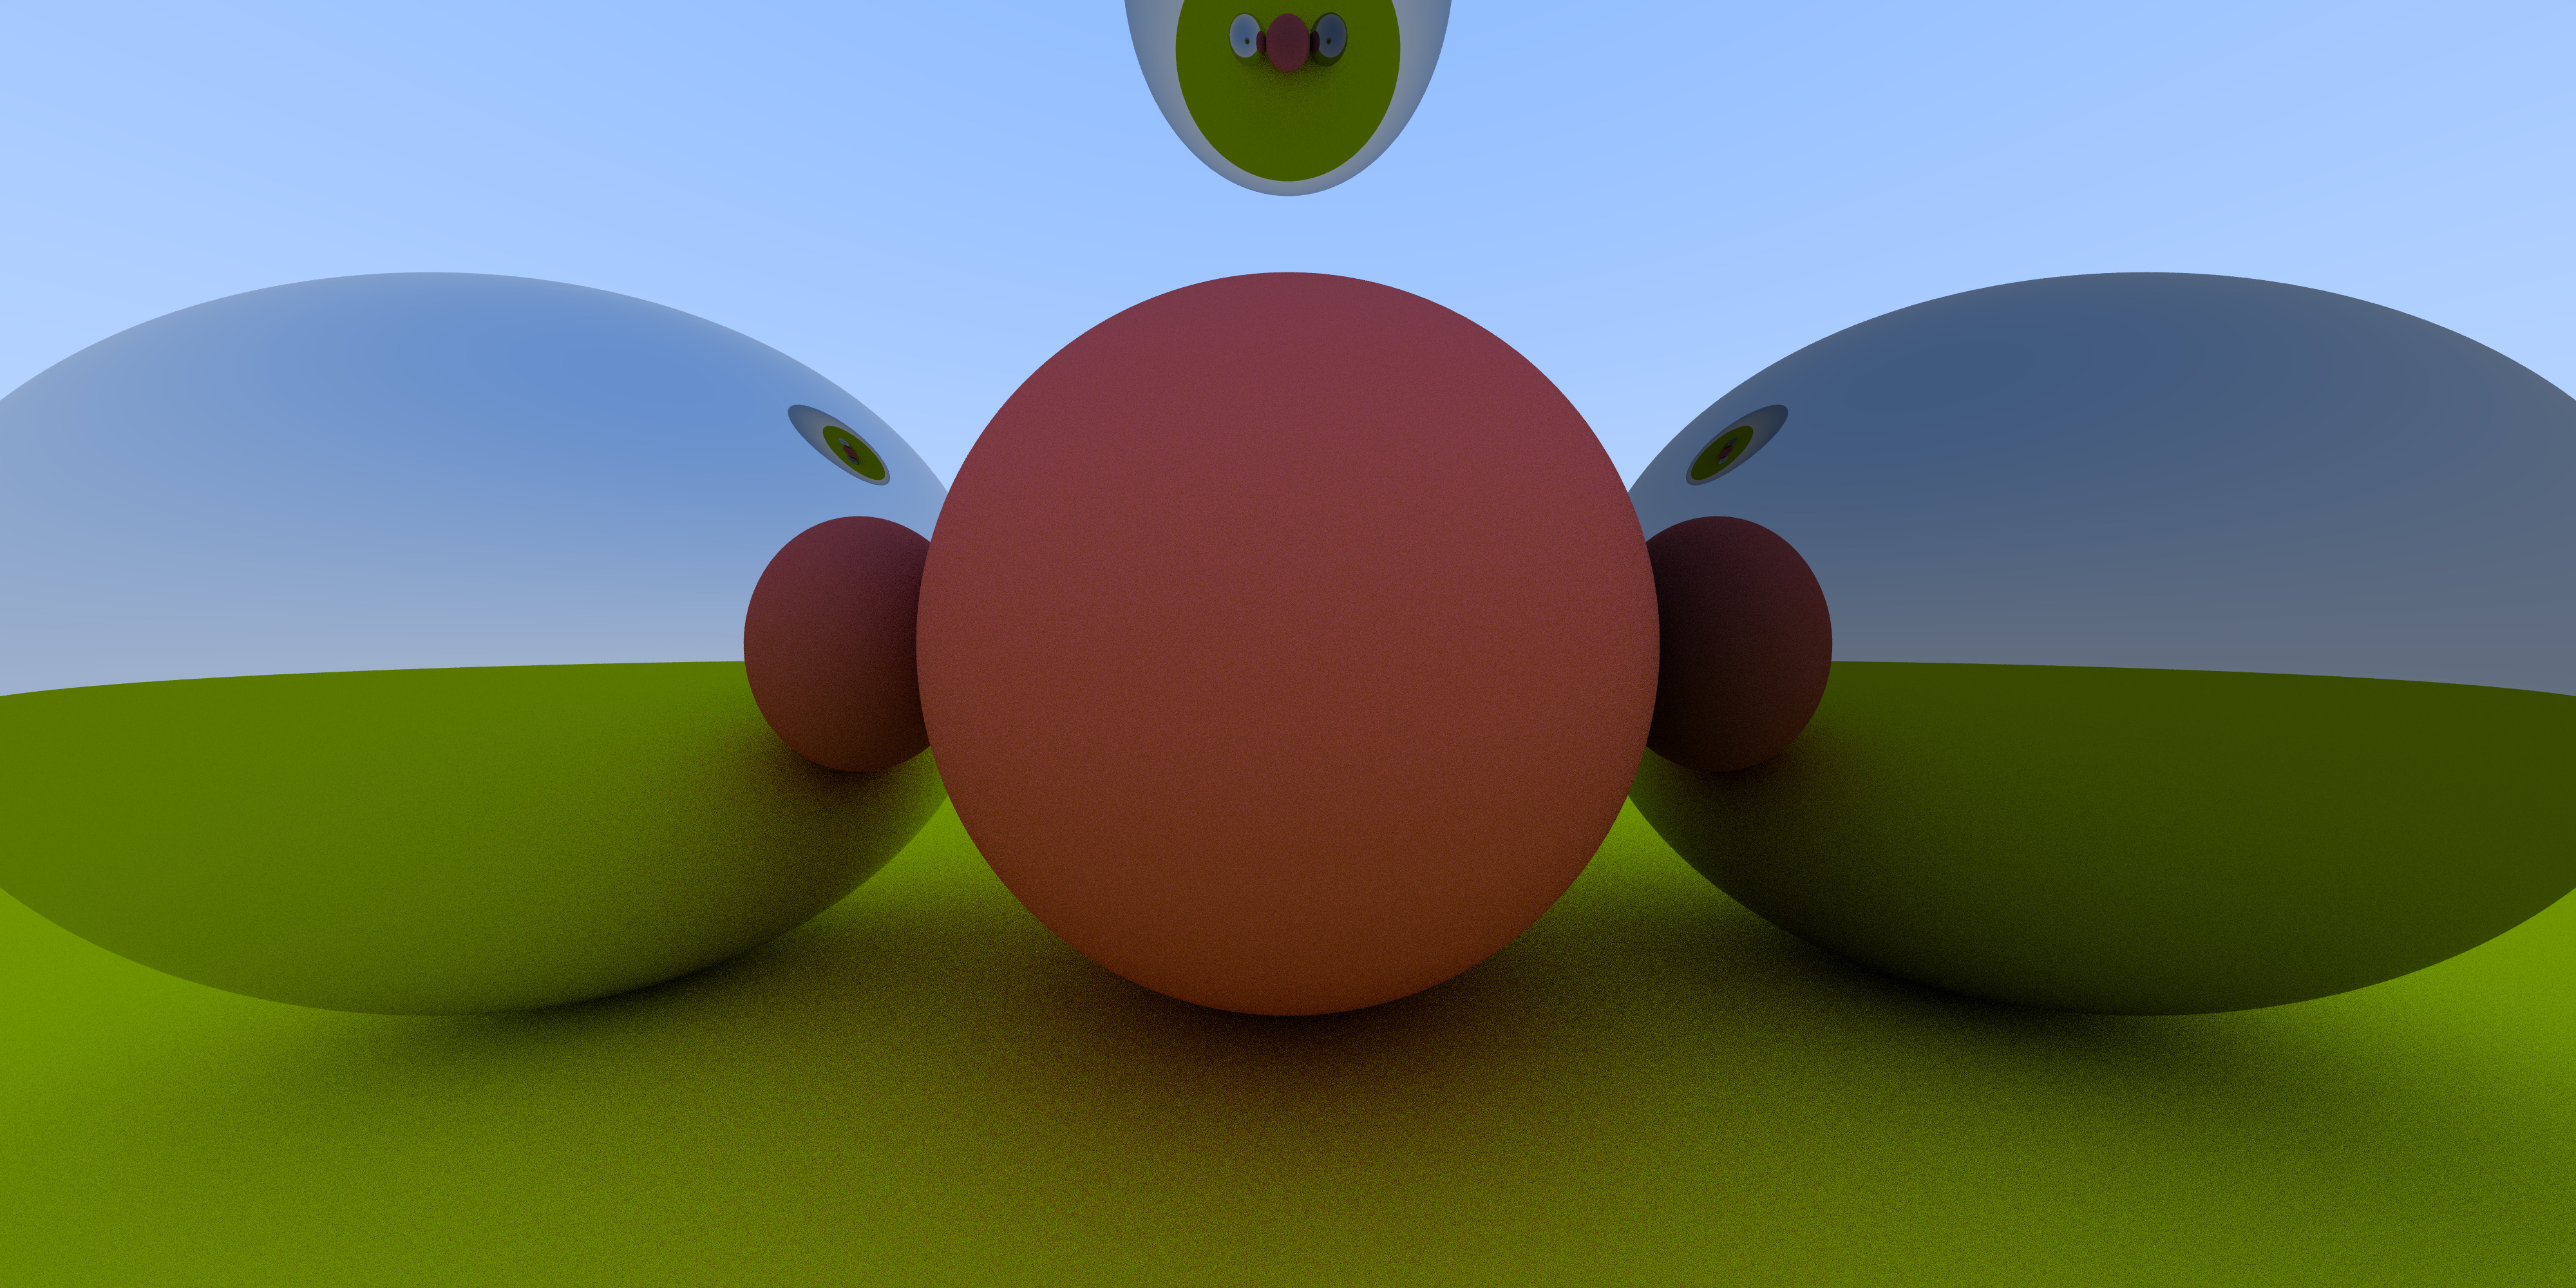
\includegraphics[width=\linewidth]{fiveSpheres.jpg}
\end{frame}

\begin{frame}
	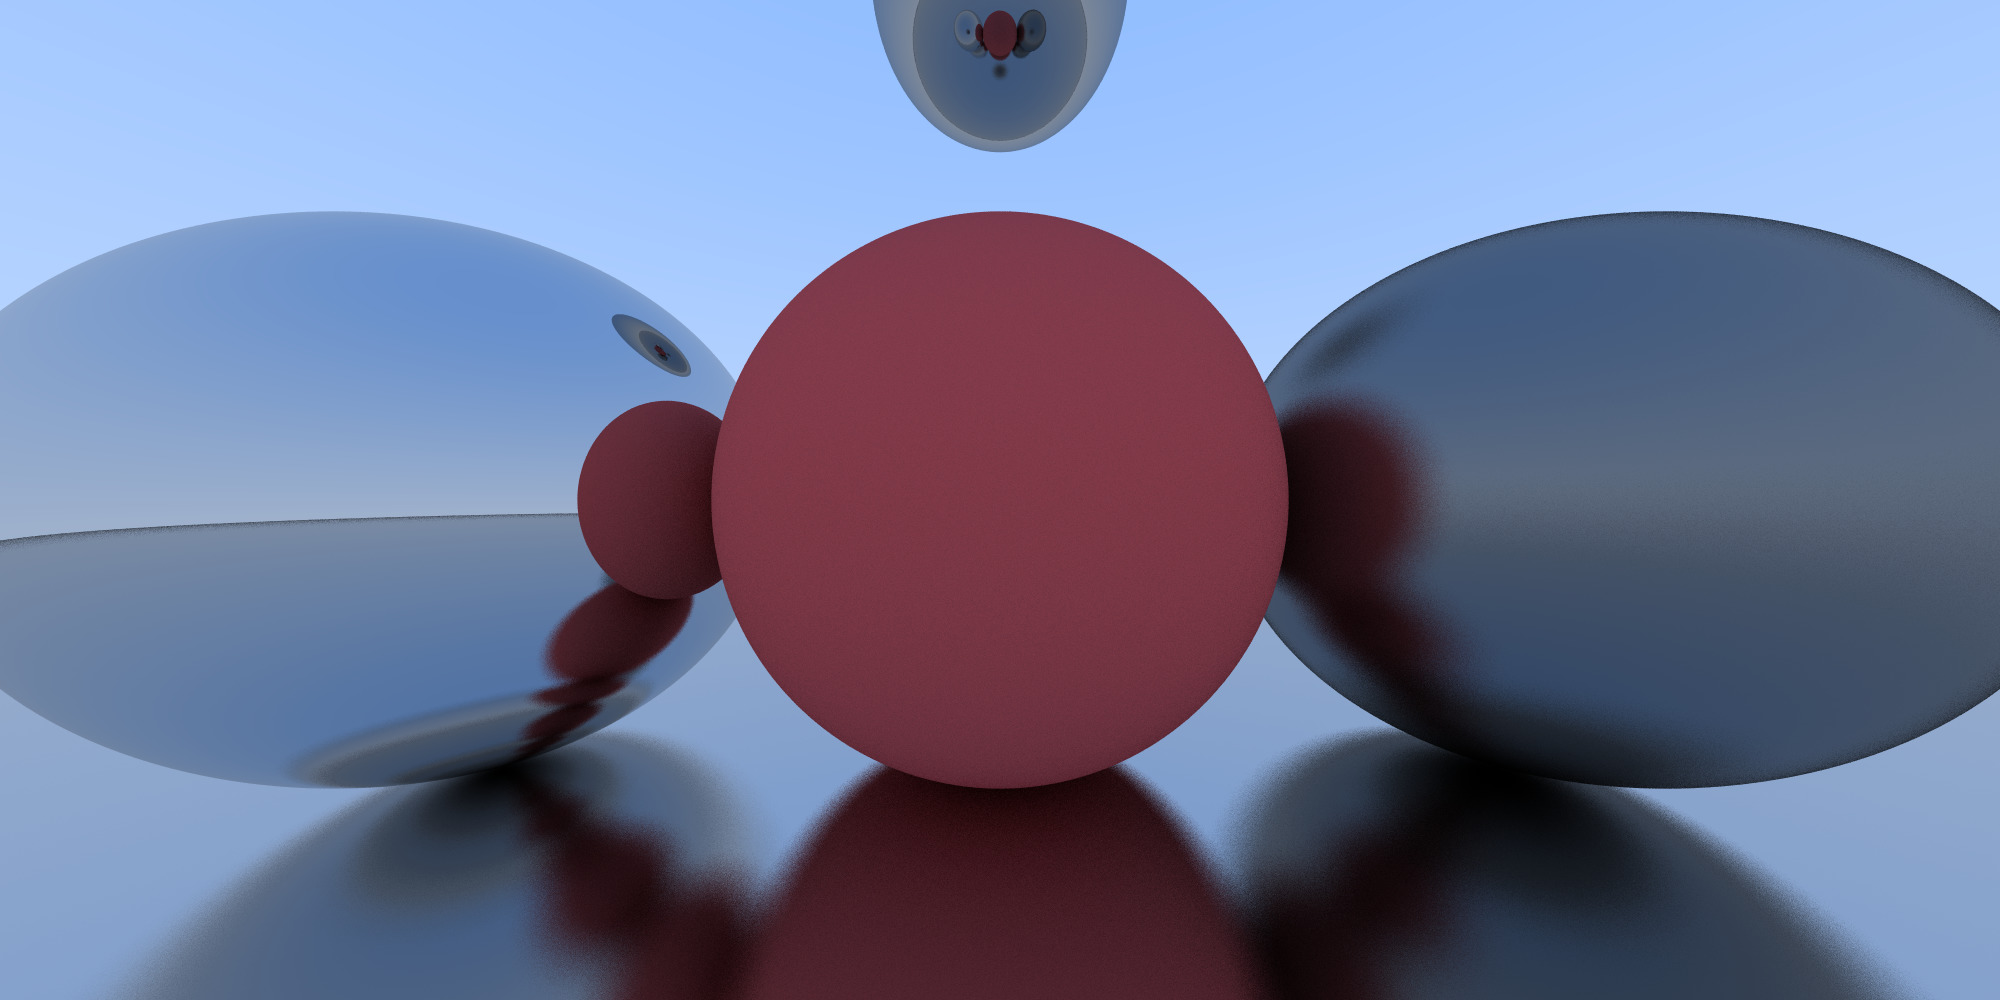
\includegraphics[width=\linewidth]{fuzemetal.jpg}
\end{frame}
\begin{frame}
	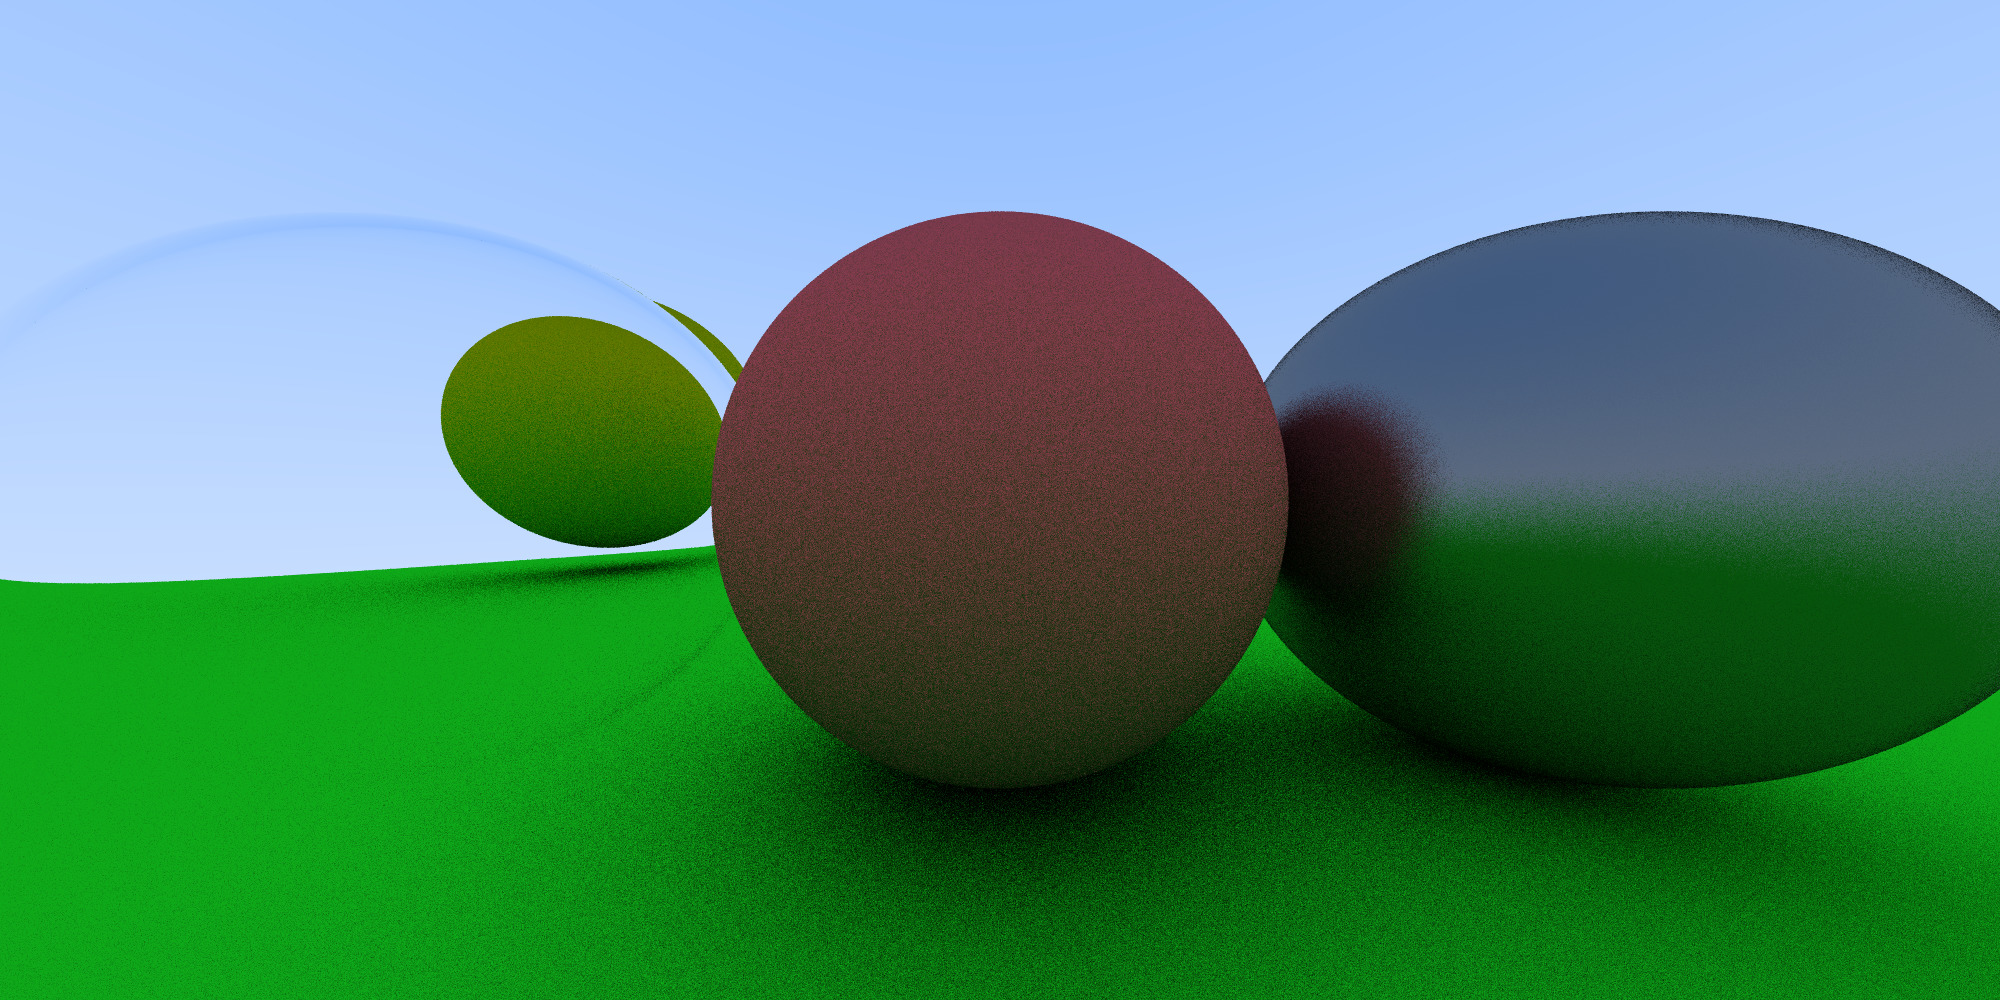
\includegraphics[width=\linewidth]{sec.jpg}
\end{frame}

%------------------------------------------------
\end{document}
